\subsection{基于硬件调整的温度值标定调试}
通过调整可变电阻VR1的值,改变温度传感器读取的数值。从$28.6\textcelsius$调整为$31.0\textcelsius$。
\begin{table}[H]
  \centering
  \caption{温度值标定调试结果}
  \begin{tabular}{L{0.4\textwidth}C{.4\textwidth}}
    \toprule
    项目  & 测量值\\
    \midrule
    当前实际室温  & 31.1\textcelsius \\
    经你完成调试后测试程序显示温度  & 31.0\textcelsius \\
    是否存在严重的元器件离散性问题?  & 否\\
    \bottomrule
  \end{tabular}
\end{table}
\subsection{基于软件后处理的电流数据标定}
利用多组数据,通过线性回归计算出软件读取值与实际值的线性关系,从而在软件层面实现数据矫正。
通过串接电子负载,可以调整USB接口输出的电流值,从而得到多组数据。
\begin{table}[H]
\centering
\caption{采样得到的电流数据}
\begin{tabular}{C{.4\textwidth}C{.4\textwidth}}
  \toprule
  Val(串口读取值) & I(实际值)\\
  \midrule
  457mA & 78.3mA\\
  609mA & 105.0mA\\
  \bottomrule
\end{tabular}
\end{table}
可见串口读取值与实际值有较大偏差,通过计算直线方程得
\begin{equation*}
y = 0.1737x - 1.021
\end{equation*}
\begin{lstlisting}[language=C++,caption={修改过后的代码},captionpos=b]
  Serial.print("Socket #1 current: ");
  Serial.print((float)Sensor0*0.173793-1.02102156);
  Serial.print(" mA");
  Serial.print("\t\t");
  Serial.print("Socket #2 current: ");
  Serial.print((float)Sensor1*0.1754680838-2.017431873);
  Serial.println(" mA");
\end{lstlisting}
利用标定好的程序进行测量
\begin{table}[H]
  \centering
  \caption{重新测量并计算误差}
  \begin{tabular}{C{.3\textwidth}C{.3\textwidth}C{.2\textwidth}}
    \toprule
    Val(串口读取值) & I(实际值) & 误差\\
    \midrule
    109.34 & 108.9 & 0.40\%  \\
    93.87  & 93.5  & 0.40\%  \\
    122.89 & 122.9 & 0.01\% \\
    139.49 & 139.5 & 0.01\% \\
    156.09 & 155.7 & 0.25\%  \\
    181.29 & 181.6 & 0.17\% \\
    232.04 & 230.9 & 0.49\%  \\
    384.28 & 382.4 & 0.49\% \\
    \bottomrule
  \end{tabular}
  \end{table}
可见误差已经很小了,仿照1的过程,我们也完成了另一条电路的标定。
\section{软硬件相结合的系统调试}
\subsection{测试任务一}
\begin{table}[H]
\centering
\caption{测试任务1}
\begin{tabular}{L{.2\textwidth}L{.3\textwidth}L{.3\textwidth}}
  \toprule
  输出命令  & 1\#和2\#插座的状态  & 控制电压\\
  \midrule
  发送字符A & 智能插座1\#插座的输出电压,P1的电压:\underline{5.138}V  & J3的\underline{L1}脚电压:\underline{2.925}V\\
  发送字符a & 智能插座1\#插座的输出电压,P1的电压:\underline{0}V  & J3的\underline{L1}脚电压:\underline{0}V\\
  发送字符B & 智能插座2\#插座的输出电压,P2的电压:\underline{5.127}V  & J3的\underline{L2}脚电压:\underline{2.929}V\\
  发送字符b & 智能插座2\#插座的输出电压,P2的电压:\underline{0}V  & J3的\underline{L2}脚电压:\underline{0}V\\
  \bottomrule
\end{tabular}
\end{table}
\subsection{测试任务二}
\begin{table}[H]
  \centering
  \caption{测试任务2}
  \begin{tabular}{L{.3\textwidth}C{.3\textwidth}L{.1\textwidth}}
    \toprule
    项目  & 测量值  & 单位\\
    \midrule
    1\#插座外接的用电器 & \multicolumn{2}{c}{小台灯} \\
    1\#插座电流值 & 196.23  & mA\\
    2\#插座外接的用电器 & \multicolumn{2}{c}{可调光台灯}\\
    2\#插座电流值(最亮时) & 210.83  & mA\\
    2\#插座电流值(最暗时) & 40.52 & mA\\
    插座电压值  & 4.918 & V\\
    温度测量值(环境温度)  & 28.62 & \textcelsius\\
    温度测量值(手指触摸温度)  & 30.3  & \textcelsius\\
    \bottomrule
  \end{tabular}
  \end{table}
\subsection{测试任务三}
将2\#插座上的可调光台灯换成风扇,并接通风扇的插座电源,测量风扇的各档工作电流值。
\begin{table}[H]
\centering
\caption{测试任务3}
\begin{tabular}{L{.3\textwidth}C{.3\textwidth}L{.1\textwidth}}
  \toprule
  项目  & 测量值  & 单位\\
  \midrule
  风扇慢速档电流值 &  239.51  & mA\\
  风扇中速档电流值 &  361.16  & mA\\
  风扇快速档电流值 &  422.51  & mA\\
  \bottomrule
\end{tabular}
\end{table}
\begin{figure}[H]
  \centering
  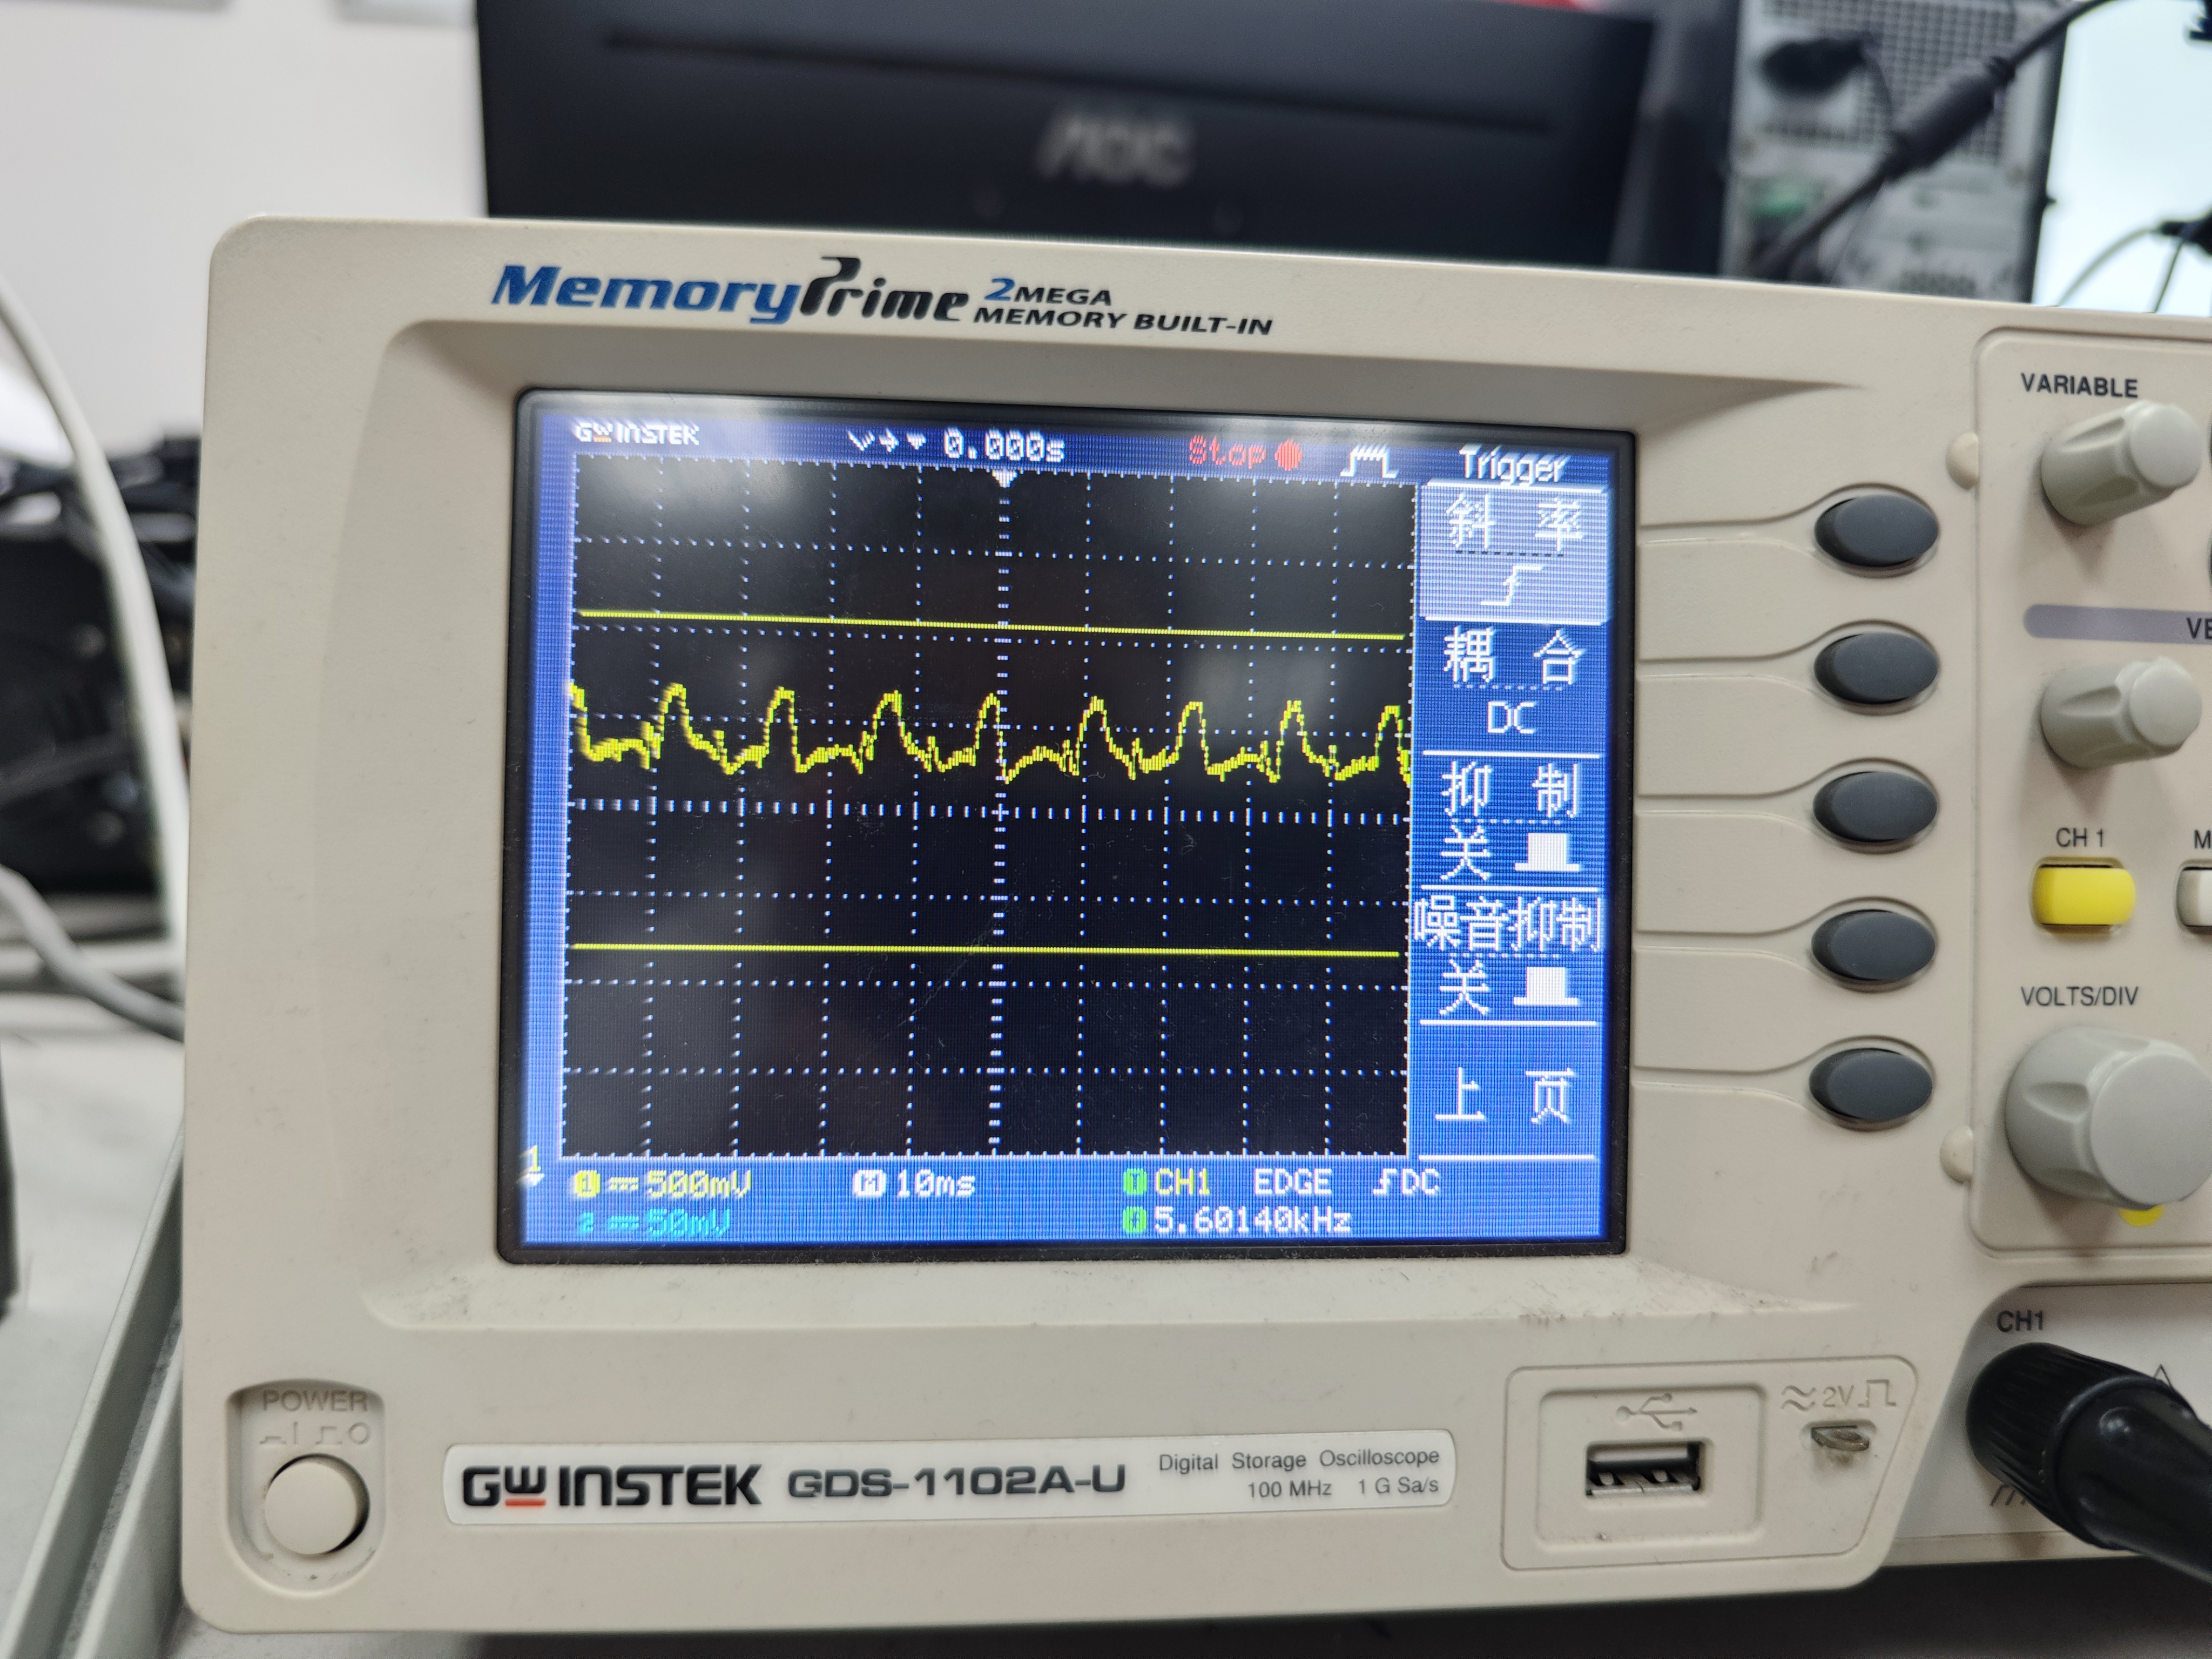
\includegraphics[width=.7\textwidth]{./figures/插座/PWM.jpg}
  \caption{风扇电流值呈周期性变化}
\end{figure}
在测量可调光小台灯及风扇电流的时候,发现其电流一直处于波动状态,可能是因为其使用了PWM技术,导致电流处于周期性波动。
\subsection{软硬件联调任务一}
在智能插座给风扇供电时,电流值不停地大小波动变化,这是风扇采用了PWM技术。为了使得测得的风扇电流趋于平稳,我们采用了\textbf{选择移动平均法}进行电流的处理。
通过\verb|float currents[16]|记录近16个电流值并求取平均值,经测试,这样可以使电流在同一挡位中平稳,并在挡位切换时快速响应。
\begin{lstlisting}[language=C++, caption={任务一}, captionpos=b]
float currents_1[16];//任务一的代码,通过计算最近的16个数值求平均来抹平波动
int head_1 = 0;
float currents_2[16];
int head_2 = 0;
float sum;
//以上是变量声明
Sensor0 = Sensor0 * 0.173793 - 1.02102156;
Sensor1 = Sensor1 * 0.1754680838 - 2.017431873;
currents_1[head_1] = Sensor0;
head_1 = (head_1 + 1) % 16;
sum = 0;
for (int i = 0; i < 16; i++)
{
  sum += currents_1[i];
}
sum /= 16.0;
// send sensor values:
Serial.print("Socket #1 current: ");
Serial.print((float)sum);
Serial.print(" mA");
Serial.print("\t\t");
currents_2[head_2] = Sensor0;
head_2 = (head_2 + 1) % 16;
sum = 0;
for (int i = 0; i < 16; i++)
{
  sum += currents_2[i];
}
sum /= 16.0;
Serial.print("Socket #2 current: ");
Serial.print((float)sum);
Serial.println(" mA");
//以上这段放在loop函数中来实现电流的计算和输出
\end{lstlisting}
\subsection{软硬件联调任务三}
本任务采用板载LED进行调试,当按下SW1,智能插座电压被分压,导致电压下降。
本任务通过改变LED灯的变换来调试输出电压下降的情况。
\begin{lstlisting}[language=C++, caption={任务三}, captionpos=b]
if(Sensor2 < 4800)//任务三的代码,Sensor2采集的电压值即为智能插座的电压值
{
  digitalWrite(pinLED,HIGH); //D4亮
}else
{
  digitalWrite(pinLED,LOW); //D4灭
}
  \end{lstlisting}
``供电电压突然下降''时,小台灯必须处于点亮状态,若小台灯不点亮则该支路没有电流,分压电阻无法分压,电压将不会有变化。
\subsection{关于按钮}
\begin{table}[H]
\centering
\caption{按钮电压与程序读出值}
\begin{tabular}{L{.3\textwidth}L{.4\textwidth}C{.2\textwidth}}
  \toprule
  检测项目  & 检测结果 & s1按钮的程序读取值(0/1)\\
  \midrule
  电路上电,按下S1按钮并保持,测量S1电平:  & S1脚的电平\underline{3.313}V。这个就是在按下按钮状态下,系统能通过软件检测到的信号。  & 1\\
  电路上电,松开S1按钮,测量S1电平:  & S1脚的电平\underline{0}V。这个就是在松开按钮状态下,系统能通过软件检测到的信号。  & 0\\
  \bottomrule
\end{tabular}
\end{table}